\documentclass{latex/webofc}
\usepackage[varg]{txfonts}   % Web of Conferences font
\usepackage{amsmath,bm}
\usepackage{hyperref}
\graphicspath{{figures/}}
\usepackage{listings}
\RequirePackage{caption}
\RequirePackage{subcaption}  % Needed for subfigures
\usepackage[cache=false,newfloat=true,finalizecache]{minted}
\usepackage[capitalize]{cleveref}% https://ctan.org/pkg/cleveref % Must be loaded after hyperref
\usepackage{lineno}
\usepackage{lmodern}% https://www.ctan.org/pkg/lm % Use same fonts as journal submission and match layout

\usemintedstyle{friendly}
\setminted[python]{}

\hypersetup{bookmarksnumbered=true, bookmarksopen=true, bookmarksopenlevel=0}
\hypersetup{pdftitle={Bayesian Methodologies with pyhf}, pdfauthor={Matthew Feickert, Lukas Heinrich, Malin Horstman}}
\hypersetup{colorlinks,breaklinks}
\hypersetup{linkcolor=blue,citecolor=blue,filecolor=black,urlcolor=blue}

\newcommand{\HiFa}{\texttt{HistFactory}}
\newcommand{\Root}{\texttt{ROOT}}
\newcommand{\RooStats}{\texttt{RooStats}}
\newcommand{\RooFit}{\texttt{RooFit}}
\newcommand{\pyhf}{\texttt{pyhf}}
\newcommand{\CLs}{\mathrm{CL}_{s}}
% alias for which terms to be highlighted
% \newcommand\term[1]{\dotuline{\textsl{#1}}}
\newcommand{\term}[1]{\textsl{#1}}

\newcommand{\freeset}{\bm{\eta}}
\newcommand{\constrset}{\bm{\chi}}
\newcommand{\singleconstr}{\chi}

\newcommand{\channelcounts}{\bm{n}}
\newcommand{\auxdata}{\bm{a}}

\newcommand{\poiset}{\bm{\psi}}
\newcommand{\nuisset}{\bm{\theta}}

\newcommand{\fullset}{\bm{\phi}}
\newcommand{\singlefull}{\phi}

% atlasunit.sty
\newcommand*{\TeV}{\ensuremath{\text{Te\kern -0.1em V}}}
\newcommand*{\GeV}{\ensuremath{\text{Ge\kern -0.1em V}}}
\newcommand*{\MeV}{\ensuremath{\text{Me\kern -0.1em V}}}
\newcommand*{\keV}{\ensuremath{\text{ke\kern -0.1em V}}}
\newcommand*{\eV}{\ensuremath{\text{e\kern -0.1em V}}}

\newcommand*{\ifb}{\mbox{fb\(^{-1}\)}}
\newcommand*{\ipb}{\mbox{pb\(^{-1}\)}}
\newcommand*{\inb}{\mbox{nb\(^{-1}\)}}

%
\begin{document}

% CHEP proceedings are due to the conference Jan 31, 2025, have an 4-8 pages for parallel oral contributions
\linenumbers
%
\title{Building a Columnar Analysis Demonstrator for ATLAS PHYSLITE Open Data using the Python Ecosystem}

\author{\firstname{KyungEon} \lastname{Choi}\,\orcidlink{0000-0003-0748-694X}\inst{1} \and
 \firstname{Matthew} \lastname{Feickert}\,\orcidlink{0000-0003-4124-7862}\inst{2}\fnsep\thanks{Corresponding author \email{matthew.feickert@cern.ch}
\\Copyright 2024 CERN for the benefit of the ATLAS Collaboration.
Reproduction of this article or parts of it is allowed as specified in the CC-BY-4.0 license.} \and
 \firstname{Nikolai} \lastname{Hartmann}\,\orcidlink{0000-0003-0047-2908}\inst{3} \and
 \firstname{Lukas} \lastname{Heinrich}\,\orcidlink{0000-0002-4048-7584}\inst{4} \and
 \firstname{Alexander} \lastname{Held}\,\orcidlink{0000-0002-8924-5885}\inst{2} \and
 \firstname{Evangelos} \lastname{Kourlitis}\,\orcidlink{0000-0001-6568-2047}\inst{4} \and
 \firstname{Nils} \lastname{Krumnack}\inst{2} \and
 \firstname{Giordon} \lastname{Stark}\,\orcidlink{0000-0001-6616-3433}\inst{5} \and
 \firstname{Matthias} \lastname{Vigl}\,\orcidlink{0000-0003-2281-3822}\inst{4} \and
 \firstname{Gordon} \lastname{Watts}\,\orcidlink{0000-0002-0753-7308}\inst{6}
 on behalf of the ATLAS Computing Activity
}

\institute{University of Texas at Austin, Austin, Texas, USA
 \and
 University of Wisconsin-Madison, Madison, Wisconsin, USA
 \and
 Ludwig Maximilians Universitat, Munich, Germany
 \and
 Technical University of Munich, Munich, Germany
 \and
 Santa Cruz Institute for Particle Physics, Santa Cruz, California, USA
 \and
 University of Washington, Seattle, Washington, USA
}

\abstract{%
 The ATLAS experiment is in the process of developing a columnar analysis demonstrator, which takes advantage of the Python ecosystem of data science tools.
This project is inspired by the analysis demonstrator from IRIS-HEP.
The demonstrator employs PHYSLITE OpenData from the ATLAS collaboration, the new Run 3 compact ATLAS analysis data format.
The tight integration of ROOT features within PHYSLITE presents unique challenges when integrating with the Python analysis ecosystem.
The demonstrator is constructed from ATLAS PHYSLITE OpenData, ensuring the accessibility and reproducibility of the analysis.
The analysis pipeline of the demonstrator incorporates a comprehensive suite of tools and libraries.
These include uproot for data reading, awkward-array for data manipulation, Dask for parallel computing, and hist for histogram processing.
For the purpose of statistical analysis, the pipeline integrates cabinetry and \texttt{pyhf}, providing a robust toolkit for analysis.
A significant component of this project is the custom application of corrections, scale factors, and systematic errors using ATLAS software.
The infrastructure and methodology for these applications will be discussed in detail during the presentation, underscoring the adaptability of the Python ecosystem for high-energy physics analysis.

}
%
\maketitle
%

\section{Introduction}\label{sec:introduction}

As the High Luminosity LHC (HL-LHC) era approaches, the ATLAS experiment~\cite{PERF-2007-01} has been preparing software and computing upgrades to address the challenges and opportunities outlined in the ATLAS Software and Computing HL-LHC Roadmap~\cite{CERN-LHCC-2022-005}.
From the 2022 computing model projections, ATLAS does not anticipate being able to store all analysis computations on disk, as even under the ``aggressive'' R\&D scenario, sustained year-on-year budget increases of more than 10\% would be required to meet the disk storage quota required, as seen in~\Cref{fig:atlas-disk-projection}.
To prepare for this reality, ATLAS has begun to explore strategies of trading disk for compute by performing ``on-the-fly'' computations for analysis quantities when possible, rather than reading them from disk.
This approach is supported by the design decisions of PHYSLITE --- the common file format for the ATLAS Run 4 Analysis Model~\cite{Schaarschmidt:2024vzr}.
PHYSLITE is a monolithic file format --- intended to support around 80\% of all physics analyses in Run 4 --- that contains already-calibrated physics objects for fast analysis, and allows for direct support without the need to create derived ROOT ntuples for analysis.

% The ATLAS experiment is in the process of developing a columnar analysis demonstrator, which takes advantage of the Python ecosystem of data science tools

Great introductions here~\cite{CERN-LHCC-2022-005,nanobind}.

\begin{figure}
    \centering
    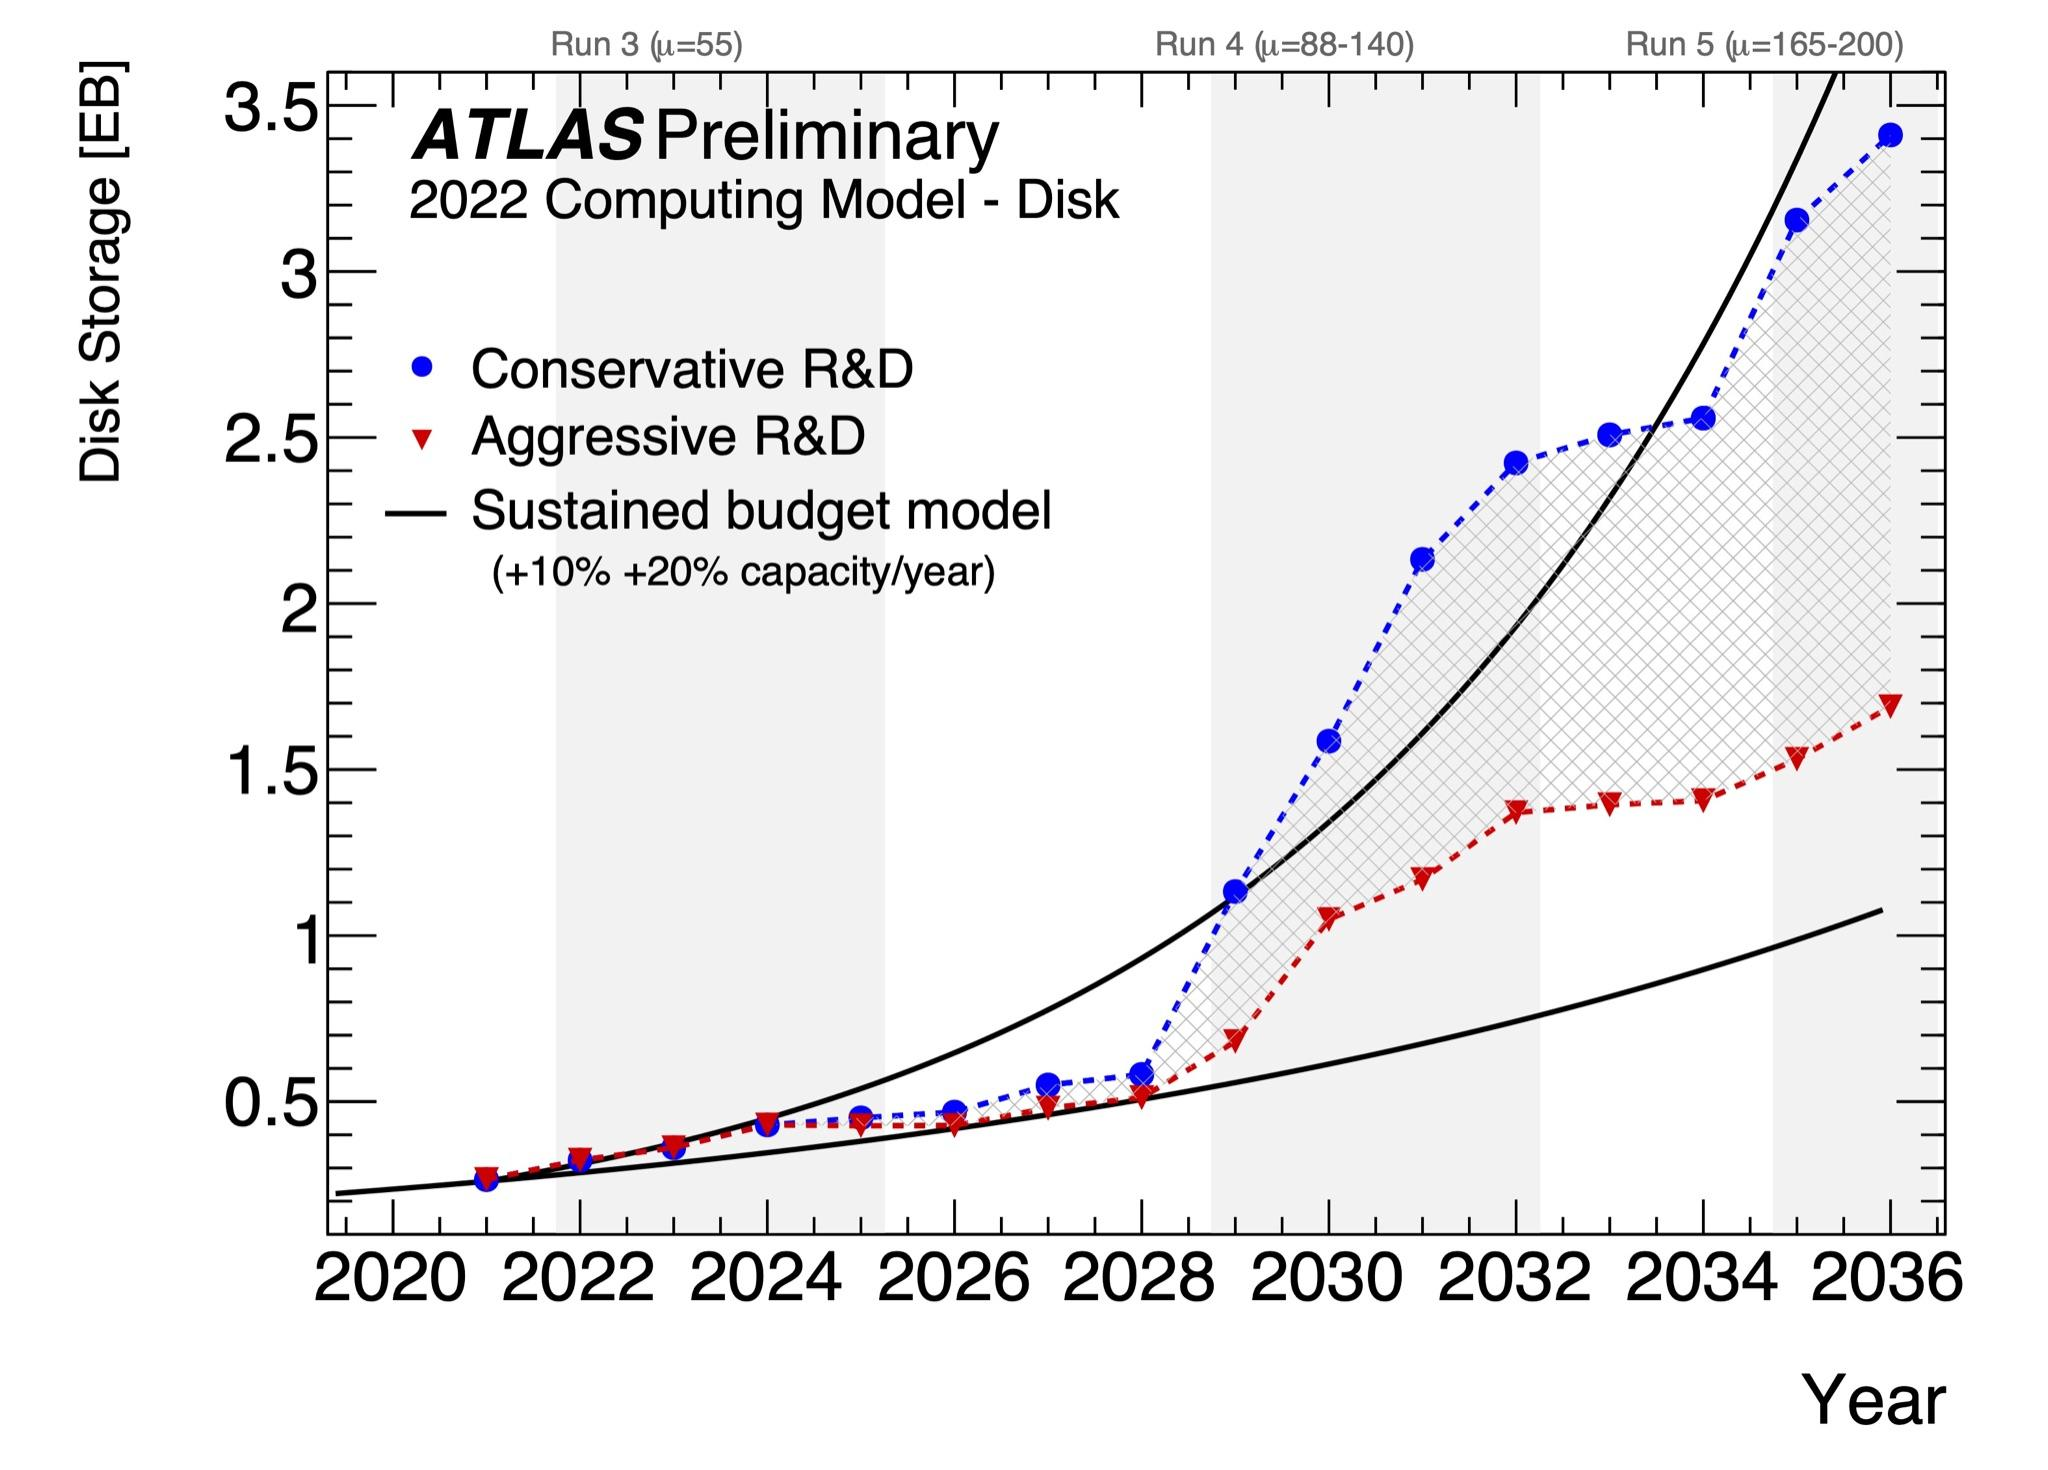
\includegraphics[width=0.8\textwidth]{atlas-disk-projection.png}
    \caption{Projected evolution of disk usage from 2020 until 2036, under the conservative (blue) and aggressive (red) R\&D scenarios.
The grey hatched shading between the red and blue lines illustrates the range of resources consumption if the aggressive scenario is only partially achieved.
The black lines indicate the impact of sustained year-on-year budget increases, and improvements in new hardware, that together amount to a capacity increase of 10\% (lower line) and 20\% (upper line).
The vertical shaded bands indicate periods during which ATLAS will be taking data.~\cite{CERN-LHCC-2022-005}}
    \label{fig:atlas-disk-projection}
\end{figure}

\section{Preliminary Performance Tests and Future Decisions and Work}\label{sec:conclusions}

During the ongoing refactor for the \texttt{v2} prototype, preliminary integrated benchmarks have been created to measure the time spent in each tool per event (excluding I/O) in comparison with the xAOD model.
While direct one-to-one comparisons are not possible given the inherent differences in data processing, the tests have been designed to be as close as possible.
The benchmarks compare the same version of each cP tool, only use the \texttt{C++} code (no Python is involved so as to isolate the \texttt{C++} performance), and the time for the xAOD model includes the event store access overhead (which is per-event for the xAOD model and per-batch for the columnar model).
The time for I/O and connecting columns is also not included in the performance comparisons, as this has not been optimized in the current tests and will not provide useful information, and so are removed from the benchmark.
The benchmarks show substantial speedups for the migrated tools with the columnar implementations ranging from being \emph{2-4x faster} than the xAOD interface.
The specific reasons for the speedups are currently being investigated fully, but preliminary checks show a relation with EDM access (columnar tools need to access the EDM once per event batch).

ATLAS CP tools were created 10-15 years ago to run in an analysis framework.
Battle tested, extremely well understood, excellent physics performance, strong desire to be maintained.
Rewrite cost is currently too high across collaboration to move to \texttt{correctionlib} paradigm.
Columnar cracks open ``black box'' implementations of tools for the new analysis model.
Legacy code decisions highlight columnar prototype design decisions and opportunities during tool migration.
Raises the question: ``What would it take to get to \texttt{python -m pip install atlascp}?''
Columnar prototype explores these possibilities.
Steps beyond: Modularization to level that allows packaging with \texttt{scikit-build-core}.



\section{Acknowledgements}\label{sec:acknowledgements}

Matthew Feickert, Alexander Held, and Gordon Watts are supported by the U.S. National Science Foundation (NSF) under Cooperative Agreement OAC-1836650 and PHY-2323298 (IRIS-HEP).
Lukas Heinrich and Evangelos Kourlitis are supported by the Excellence Cluster ORIGINS, which is funded by the Deutsche Forschungsgemeinschaft (DFG, German Research Foundation) under Germany's Excellence Strategy - EXC-2094-390783311 and by the German Federal Ministry of Education and Research Project 05H2021 (ErUM-FSP T02) - ``Run 3 von ATLAS am LHC: Analysis Infrastructure for the ATLAS Detektor at the LHC''.


% Don't use \bibliographystyle
% the style is already called in woc.bst, so ensure it is in the top level directory
\bibliography{bib/ref}

\end{document}

<div id='footer'><table width='100%'><tr><td class='right'><a href='http://fusioninventory.org/'><span class='copyright'>FusionInventory 9.1+1.0 | copyleft <img src='/glpi/plugins/fusioninventory/pics/copyleft.png'/>  2010-2016 by FusionInventory Team</span></a></td></tr></table></div>
